%\documentclass{scrreprt}
%\documentclass[a4paper,12pt,twoside,openany]{book}
\documentclass[a4paper]{scrreprt}

\usepackage[utf8]{inputenc}
\usepackage{enumerate}
\usepackage[english]{babel} 
\usepackage{textcomp}

\usepackage{amsmath}
\usepackage{amsfonts}
\usepackage{amssymb}
\usepackage{amsthm}
\usepackage{mathtools}

\usepackage{subcaption}

\usepackage{graphicx}
\usepackage{wrapfig}
\usepackage{caption}

\usepackage[hidelinks]{hyperref}

\newcommand{\wrapfig}[5] {
	\begin{wrapfigure}{#2}{#3\textwidth}
	\centering
	\includegraphics[width=#4\textwidth]{resources/#1}
	\caption*{#5}
	\end{wrapfigure}
}

\begin{document}

\title{Roux, an advanced approach to cubing}
\author{Dominic Zimmer}
\maketitle 

\tableofcontents
\chapter{Prologue}

\section{Abstract}
I'm going to introduce, explain, and discuss a method to solve the Rubiks Cube called \emph{Roux}. I will not assume the reader knows to how to solve the Rubiks Cube. However the geometric understanding of the cube is useful. Thus I will also mention some very basic information which might seem redundant to others.
%possible rewrite
After I ensured we are on the same level of understanding the notation, I will first give a rough overview of what Roux is. Then I will continue by going into great detail on how to approach each step.

\section{Perspectives}
Apart from Roux, there are plenty methods out there of which I will mention the most prevalent ones.

\wrapfig{union.png}{R}{0.4}{0.3}{The four steps of using the Beginners Method}

First off, I am going to cover the \emph{Beginner's Method}, also known as \emph{Layer by Layer Method}. The Method does what the name implies: it solves the cube layer by layer. This method seems pretty intuitive to most people as it starts off by solving one face (which is easy to begin with).\par
The most common method is closely related to the Beginner's Method: \emph{Fridrich's Method} or more commonly known as \emph{CFOP}. CFOP begins by forming a \textbf{c}ross on one side, extending that cross to the \textbf{f}irst two layers, \textbf{o}rienting, and \textbf{p}ermutating the last layer (leading to its unique name). You can see how closely related it is to the Beginner's Method: The key difference is that the Beginner's Method splits building the first two layers into two seperate steps whereas CFOP does this more efficiently. There are some more methods which deserve to be named here, for instance \emph{Petrus' Method}, but I'm going to leave it at that.

\section{Notation and terminology}
\subsection{Face turns}
To be able to communicate on this abstract level of thinking, we are going to use the standart notation and terminology which I will explain below.\par
In our notation we are not going to consider the colors of the individual facelets but rather keep the cube in one orientation. Thus we can easily refer to the six faces of the puzzle as \textbf{u}p, \textbf{f}ront, \textbf{r}ight, \textbf{l}eft, \textbf{b}ack and \textbf{d}own and abbreviate them each by their initial letter. Keeping that in mind, we intuitively define the moves \emph{U}, \emph{F}, \emph{R}, \emph{L}, \emph{B} and \emph{D} as clockwise 90\textdegree\ turns of their respective face.\par
To denote the counterclockwise turn of a side, we add an apostrophe to the respective turn. If we wanted to perform a 180\textdegree\ rotation of a face, we would simply append the number two to the move.


\subsection{Observations}
For clarification: we consider a respective side of the cube to face us as we turn it. For instance \emph{U} and \emph{D} rotate opposite sides and turn in opposite directions. We certainly could also use \emph{U3} with the same logic as we defined \emph{U2} yet we would notice that \emph{U3} is the very same as \emph{U'}. We also see that \emph{R2} and \emph{R2'} result in the same turns. So would someone want to use \emph{R2'} at all? Yes - sometimes it can be useful to hint using two \emph{R'} moves over two \emph{R} moves for more efficient turning. Note how we are using uppercase letters for the basic turns. Lowercase letters are reserved for an upcoming notation.

\wrapfig{slices.png}{R}{0.35}{0.3}{From top to bottom: the middle, equatorial and standing slice}

\subsection{Slice turns, wide turns and cube rotations}
Sometimes the basic turns are inconvenient to use in a certain case, for instance if you wanted to turn the middle slice, i.e., the slice \emph{sandwiched} between the right and the left side.\par


For that reason we define the \textbf{m}iddle slice turn, the \textbf{e}quatorial slice turn and the \textbf{s}tanding slice turn. We again abbreviate them respectively with their initials. However we need to declare that \texttt{M} turns in the same direction as \texttt{L}, \texttt{E} turns in the same direction as \texttt{D}, and \texttt{S} turns in the same direction as \texttt{F}. Intuitively, we can append the earlier defined suffixes \texttt{'} and \texttt{2} with their corresponding interpretations.\par

For a similar motivation as why we introduced the slice turns, we also define \emph{wide} moves. Wide moves are pretty self-explanatory: you grab two layers by expanding a face turn by the adjacent slice. We respectively add \texttt{w} for \emph{wide} to our collection of suffixes. As we add more suffixes, we want to introduce an abbreviated form for wide moves: replacing the uppercase letter by a lowercase one.\par

The last notation we want to introduce are \emph{cube rotations}. Cube rotations require you to turn the entire cube inside your hands. We denote them as the three axes \texttt{X}, \texttt{Y} and \texttt{Z}. Again we need to clarify which axis turns in which direction: \texttt{X} turns in the same direction as \texttt{R}, \texttt{Y} turns in the same direction as \texttt{U} and \texttt{Z} turns in the same direction as \texttt{F}. Since you might run into this question: we do not differentiate between uppercase and lowercase cube rotations.


\chapter{Roux}

\section{Brief overview}

%TODO move to abstract?
Before we go into detail, I am going to give you a rough idea of how roux works.\par

\wrapfig{f2b_transparent.png}{R}{0.3}{0.3}{The First Two Blocks}

%TODO capitalize or lowercase First Block, Second Block, Last Six Edges and so on?
You start off by what is called the \emph{First Block}: you build a 1x2x3 block of one color around the matching center. Next, we will mirror the first block onto the opposite side. This leaves us in the state of the \emph{First Two Blocks} already solved. If we were looking from the front side, we would see that we are left with a T-shaped area which is yet to be solved. Notice how every piece that is yet to be solved is on either the middle slice or the upper layer. Mathematicians like to call these pieces the \emph{(linear) span}, denoted as $\langle M, U \rangle$, of the turns \texttt{U} and \texttt{M}.\par

\wrapfig{lse.png}{L}{0.3}{0.3}{Before the Last Six Edges}

We now want to solve the corners of the upper layer to be left with six unsolved edges and four unsolved centers. Solving the corners of the upper layer will be split into two seperate steps. First, we orient the corners to have their common color face up. Then we permute them to the places where they belong. Both of these steps are not very trivial and thus will require some algorithms. If you want to figure some algorithms out by yourself, you usually want to try to break up the First Two Blocks and then reconstruct them slightly differently. But there is no big learning effect involved, so I would not recommend doing so.\par

As mentioned previously, we are now left with six edges and four centers unsolved. As you realize quickly, the centers are at most two \texttt{M}-slice moves from being in their correct positions, leaving us with the \emph{Last Six Edges} unsolved. You can see in the figure beside how the cube would look so far. What speeds up the process of solving the Last Six Edges is the fact that you can now solve the cube by only using algorithms of $\langle M, U\rangle$, i.e., you do not have to scramble what you have solved so far.\par

No we would like to split solving the Last Six Edges into three substeps: orienting the edges, solving the left and right upper edge, and finishing the middle slice.\par

By orienting the edges we mean that we want them to only show bottom or top layer stickers on the bottom and top layer. In our example, this would make the \texttt{U}-face only contain blue and green stickers. This can either be achieved intuitively with a little bit of practise or by folloing the patterns and steps mentioned in the according section below. Now we intuitively insert the last remaining edges on the left- and right-hand side. All that is left to do is resolving one out of four cases to finish off the middle layer.\par

Now we will precisely go into detail of each step.

\section{First block}
Our goal is to build a 1x2x3 block on our first color side. Notice that we require edges to be matching to consider the block solved. This can be achieved in various ways. I will introduce some basic concepts and leave it up to you make those more efficient.\par

You can start off by building a 1x1x2 block out of a center and edge piece. By adding more 1x1x2 blocks, you can first expand that block to a 1x2x2, then to a 1x2x3 block.\par

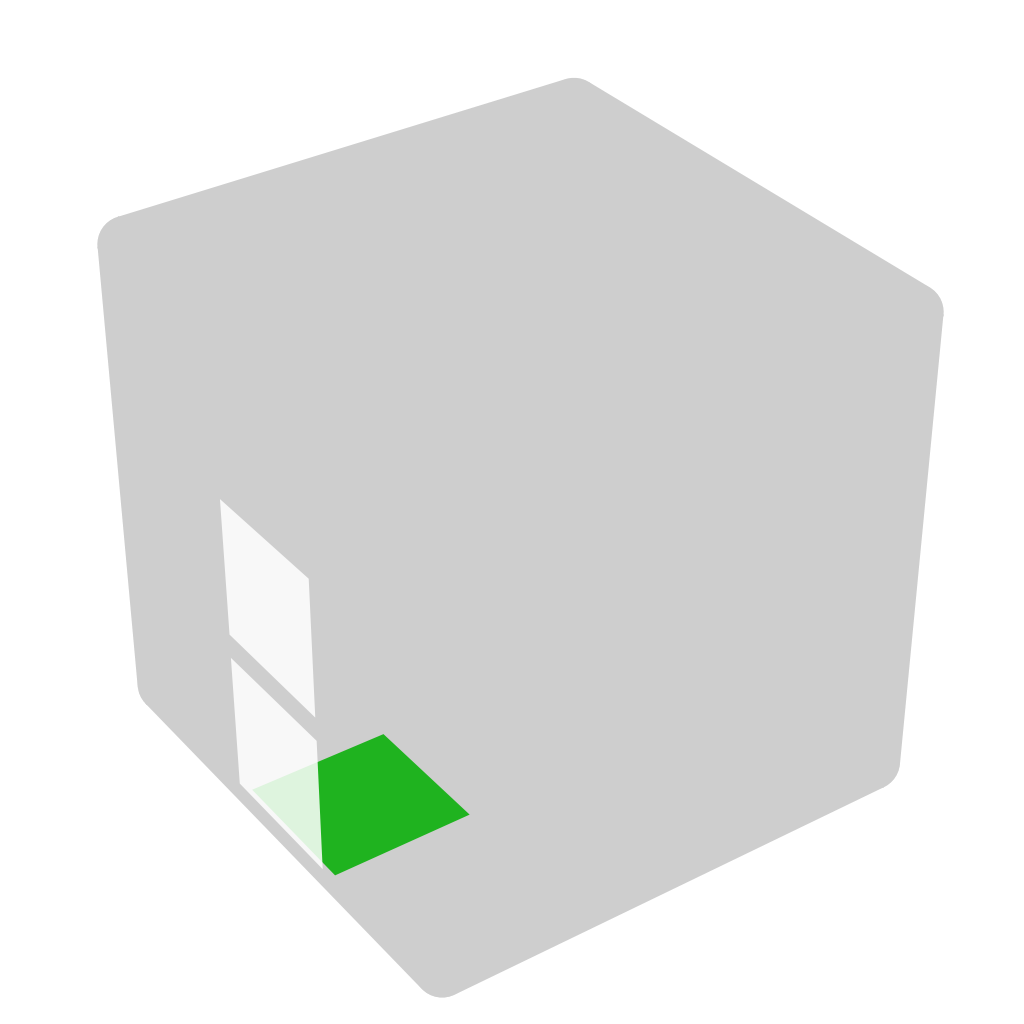
\includegraphics[height=5cm]{resources/fb_1.png}\caption{First step}
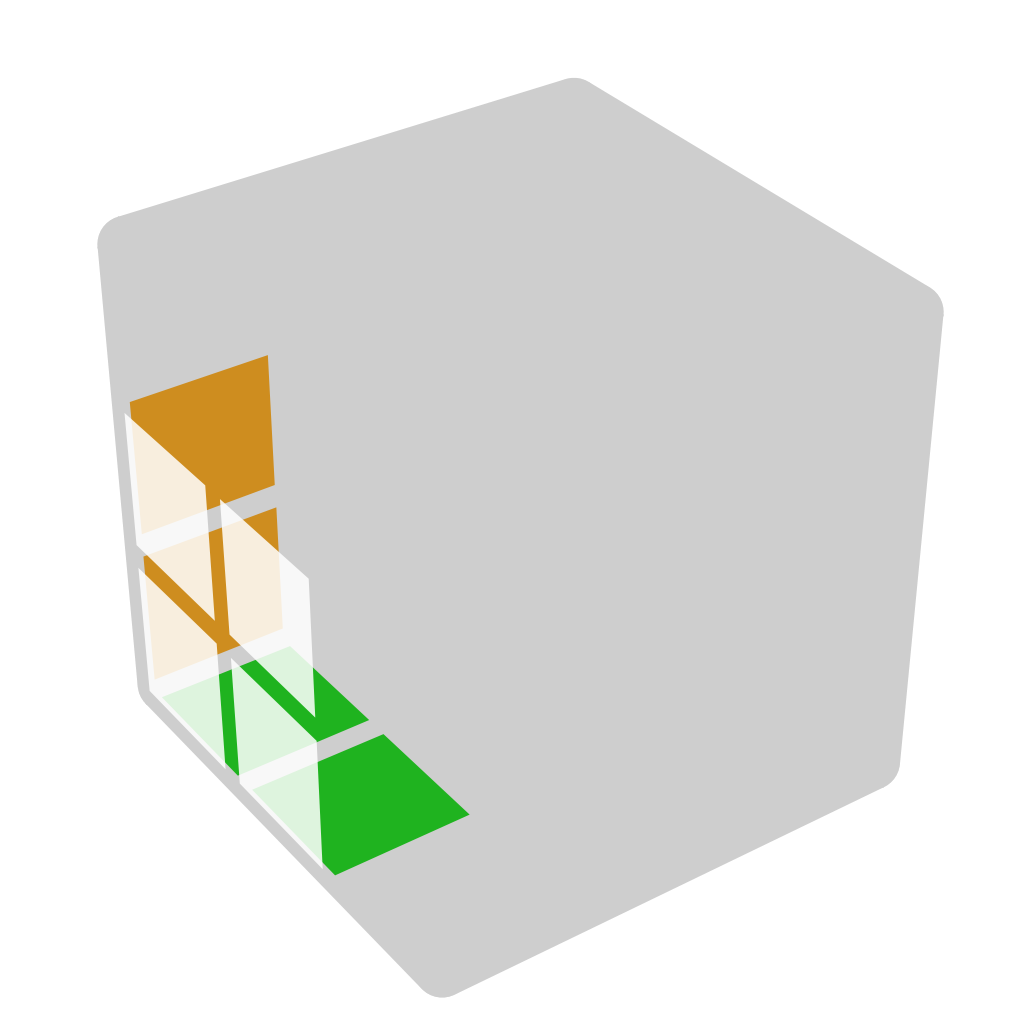
\includegraphics[height=5cm]{resources/fb_2.png}\caption{Second step}
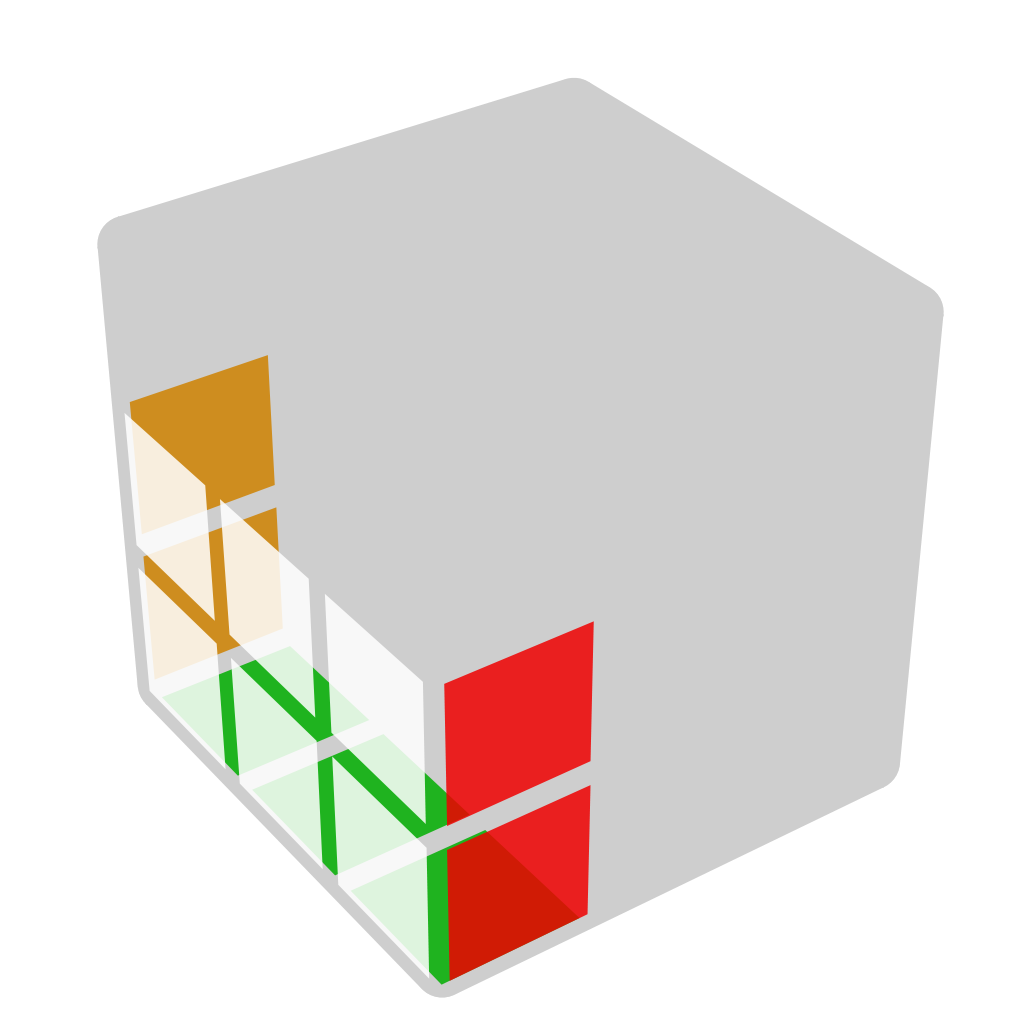
\includegraphics[height=5cm]{resources/fb_3.png}\caption{Third step}
%Alternatively, you could 


\section{Second block}

\section{Corners Last Layer}

\section{Last six edges}


\chapter{Appendix: Algorithms}

\section{2 Look CLL}

\section{CMLL}

\section{LSE}

\end{document}